\documentclass[12pt]{article}

\usepackage[english]{babel}
\usepackage[utf8x]{inputenc}
\usepackage{amsmath}
\usepackage{graphicx}
\usepackage[colorinlistoftodos]{todonotes}
\usepackage[english]{babel}
\usepackage[utf8x]{inputenc}
\usepackage{fancyhdr}
\pagestyle{fancy}
\setlength{\headheight}{15pt}
\lhead{Sharing Framework}
\rhead{Requirements Doc}
\cfoot{\thepage}

\title{\Huge{Sharing Framework}}
\author{Chris Spalding\\ Wesley Stedman\\ Bobby Kearns\\ Greg Finch\\ Ian Saad}
\date{\today}

\begin{document}
\begin{titlepage}
\maketitle
\end{titlepage}
\maketitle

\subsection{Abstract}
\textit{The Sharing Framework is implementing a database to allow users to save and share projects that they're working on. The team's use cases deal with logging on, uploading projects, saving projects, and sharing projects. Some functional requirements include what systems Edith with support as well as what might happen if the server is over capacity.}

\section{Introduction}
Edith is a code editor aimed at beginning computer programers. It uses visual tools to help coders conceptualize what the computer and code are doing when they `write' their programs. The user is able to use objects and shapes to create animations within the visual editor. From there the user is able to save, share, or load the project they are working on or have currently finished.

The Sharing Framework team is implementing a database to store the projects that are created using Edith. The database will be able to store a user's account information, as well as allow them to save and continually edit projects that are connected to their account. The team is implementing a networked database rather than a client-side saved file to avoid formatting problems that can arise from a user trying to load an unsupported file and also to allow the user to work on the project anywhere there is a computer and a network connection. This implementation allows for universal access point for the files rather than having the user always carry the file with them. 

Along with this, the database will help with implementing the functionality that allows users to share their projects. The sharing feature will allow the user to share both in progress and finished projects as long as the user saves the project to their account. In this process the site will display a url for the user to distribute via social media, email, or blogs. This will allow collaboration amongst users on a project and give a more social and creative aspect to the site. 

Although there will be no version controll implemented on the site, users that have received a link to the shared project can create their own version of the project and save it to their account. This process will allow users to make their own changes or improvements and share them with the initial sharer. This will allow users to use shared projects as a template and start their own project where they can add, delete, or improve animations in the initial project.

Without the database that can save and store a users project, no user's would be able to save a project that was too large or time consuming to finish in one sitting. Without the use of a database Edith would be a less usefull tool. With the implementation of the database users can not only save their projects whenever they are done editting, they can also access their project on any computer that has a network connection. These two features add a greater resource for editting for the user on the go.
\newpage
\section{Requirements}
\textbf{Functional Requirements and Use Cases:}
\begin{description}
\item[logging on] \hfill\\
   \textit{Actor:} Acount Holder\\
  \textit{Flow:} First the user must enter their username and password, and then click ‘login’ or an equivalent button. Server authenticates the account holder's information, allowing them to view, make, and share their projects.\\
\textit{Alternatives:} If the user doesn’t have an account then the system will prompt the user to make an account. If the user enters the wrong username/password the system will tell user and prompt them to enter username/password again.\\
\textit{Post Conditions:}
    user is logged on and can access their profile and upload/save/share docs.
\item[Saving Animations]\hfill\\
\textit{Actor:} Account Holder\\
\textit{Preconditions:} Must be logged on.\\
\textit{Flow:} Account Holder names animation and then selects save.\\
\textit{Alternatives:} if the animation has the same name as another animation, system prompts user “overwrite old file or rename?”\\
\textit{Post Conditions:} the animation is saved on the server under their username.\\
\item[Sharing Animations]\hfill\\
\textit{Actor:} Sharer\\
\textit{Preconditions/Assumptions:} User must be logged on and have a saved animation.\\
\textit{Flow:} First the Sharer logs on, then select share, then select animation to share, and finally the sharee receives URL to the animation page. The sharee cannot edit the project that has been shared\\
\textit{Alternatives:} If the sharer is not logged on the system will prompt him/her to log on. If the user has no animations to share the system will throw an error mesage telling the user "No saved projects to share".\\
\textit{PostConditions:} Return a link to animation the sharee can go to in their browser to view the animation.\\
\item[Loading From The Database]\hfill\\
\textit{Actor:} Account Holder\\
\textit{Preconditions:} The Account Holder must be logged in, have a network connection of some sort, and they must have a saved animation or project to load.\\

\textit{Flow:} The Account Holder will select which animation or project to load from database.\\

\textit{Alternatives:} If the Account Holder is not logged in, prompt them to do so. If there is no animations to load prompt them to start a new project.\\

\textit{Postconditions:} Display the animation and all the tools needed to share or edit.\\
\end{description}

\textbf{Nonfunctional Requirements}
\begin{description}
\item[Network Connection]\hfill\\
    A strong network connection between client and server is required for the functions to properly occur.
\item[What Systems We Will Support]\hfill\\
    This program will not support mobile devices.
\end{description}

On the next page you can find the UML diagram for the use cases described above.

\begin{center}
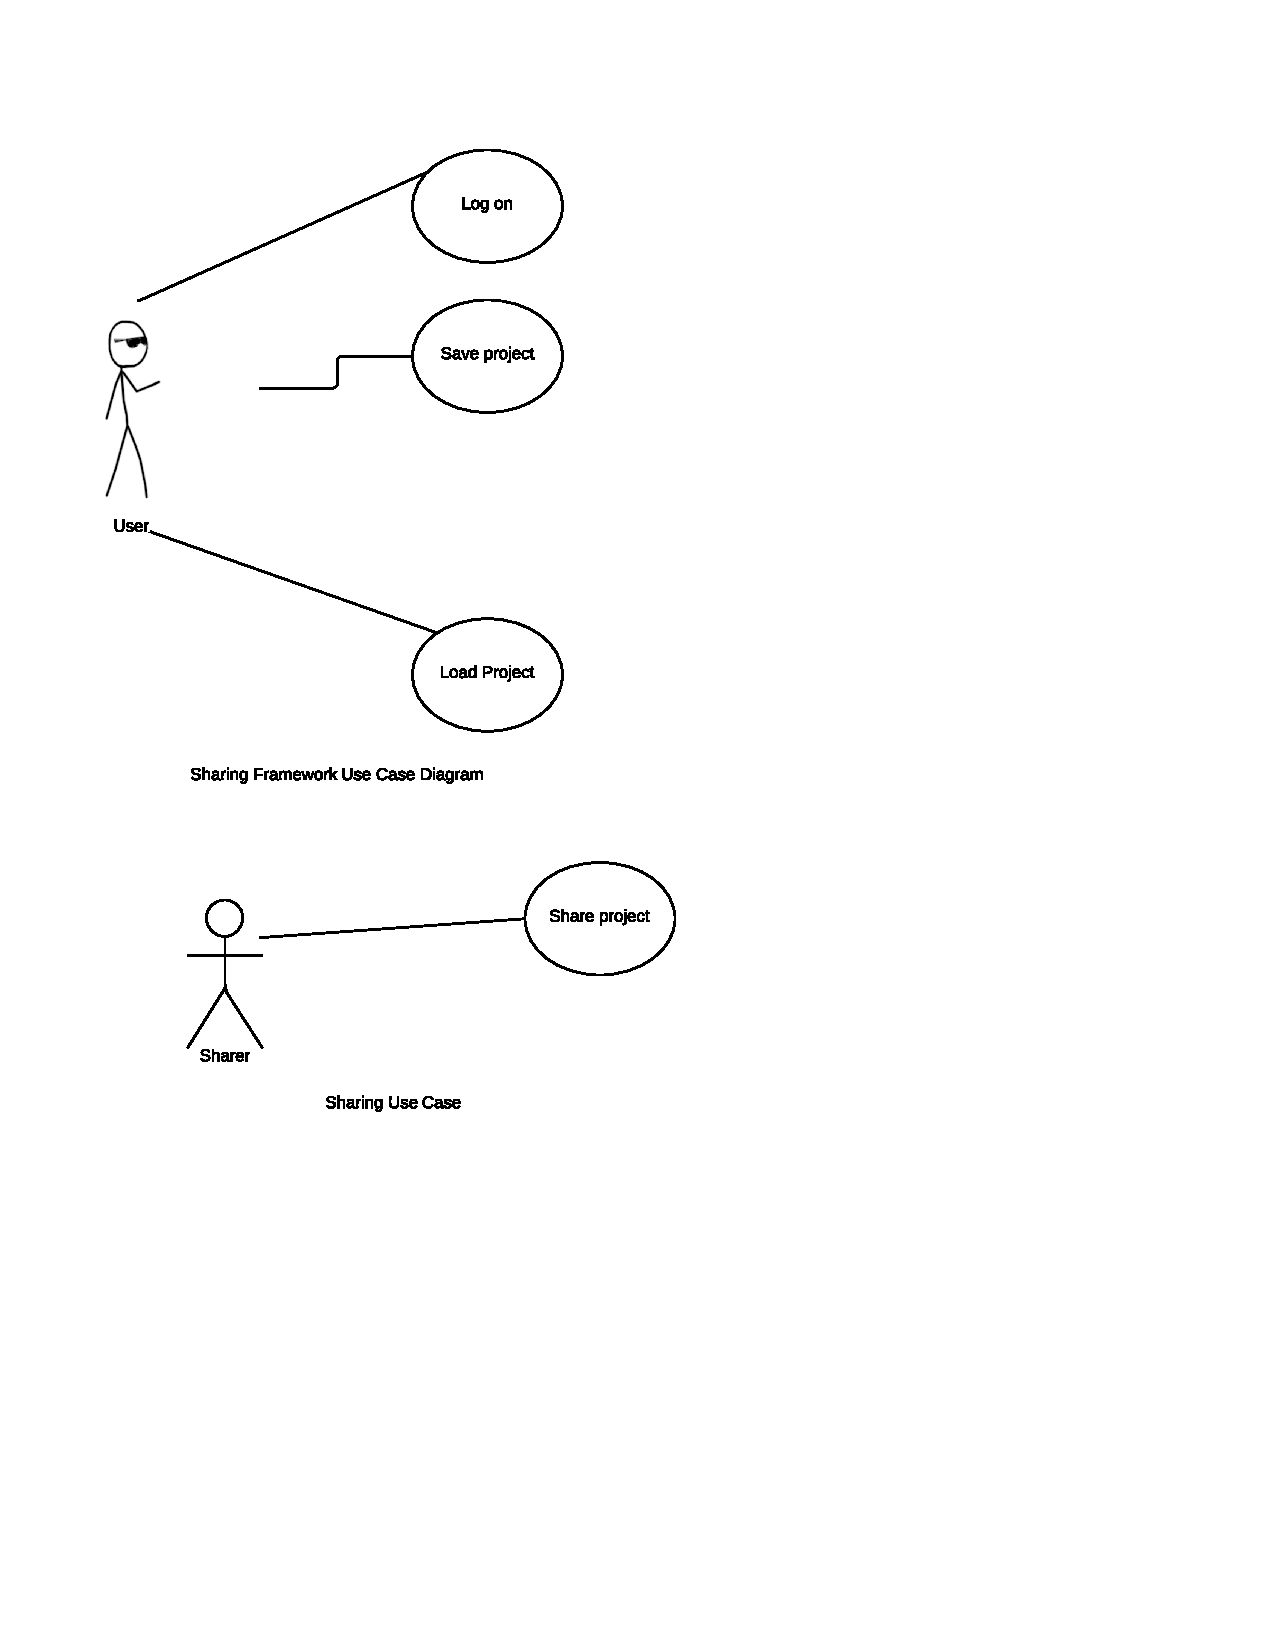
\includegraphics[scale=1]{UMLSHaringFramework}
\end{center}

\end{document}